\chapter{Analysis and Benchmark}

We profile an image of containers via cgroup and namespace
and use the seccomp mechanism to force the policy in the kernel.
We will analyze how we protect our system when hackers landing
into the container, and we profile the concurrent costs of this
mechanism.

\section{Analysis}
Our defense level is at the kernel level, but the virtual machine's
defense level is at the instruction level. Because we do not impose any
restrictions on the CPU instruction set, nor isolate the host operatin system.
Although defense level at the instruction set seems to to be more efficiency,
the virtual machine's protection consumes more time. We will show that in \ref{conc}.

In the health and medical information exchange system, the health and
medical information we protect is specialized and fixed. For example,
we do not have any attack of parsing some format string
\footnote{\url{https://owasp.org/www-community/attacks/Format_string_attack}},
which is a exploit of bypassing the ASLR \footnote{\url{https://lwn.net/Articles/569635/}}.

So we can remove some redundant system call support has reached to
limit the possibility of hacker exploitation. In order to protect
the user's data from being attacked or leaked in the information exchange system.

\subsection{Attacking Surface}
We discuessed the five stage of malware in \ref{Five_stage_of_malware}. We analyzed
three possible attack scenarios for hackers in this subsection.

\subsubsection{Administrator account leakage}
There are many situations where administrator accounts are accidentally
leaked, such as: social engineering attacks, side-channel attacks,
or account IDs and passwords known through other ways.
In 2020, 20 million household registration information in Taiwan is
suspected to be sold on the dark web\footnote{\url{https://www.ithome.com.tw/news/137955}}.

We can prevent such attacks in advance by setting up a system call filter
in seccomp. When a hacker logs into the system as a system administrator
and executes a foreign malicious program, the malicious program will call
the system out of schedule to perform malicious actions.
Even though we normally give the system administrator the highest privileges
to perform arbitrary tasks, we can analyze the behavior of the container
at build time and block unexpected behavior.

\subsubsection{Zero-day or One-day Vulnerability}
Assuming that the hacker does not have system administration privileges,
but exploits the vulnerability of the health information exchange system
(IBM/FHIR server) to conduct malicious attacks, we can also use the same
behavioral filter to filter the attack.
For example the log4j attack (CVE-2021-44228), which is a vulnerability
been published while we researching this container security issue.
Before our research, this vulnerability existed in IBM/FHIR container server
\footnote{\url{https://github.com/IBM/FHIR/issues/3156}}.
When user turns the "export to parquet" feature on, which would
brings in much of Apache Spark which leads to enable the vulnerable log4j.

But unfortunately, we have to admit that the defenses we propose cannot
withstand this log4j attack. The IBM/FHIR server itself can enable such a mechanism,
so actions using log4j are invoked at build time. We would admit these
behaviors as normal behavior in system call filter level.

\subsubsection{Breaking protection rings}

\begin{figure}
    \centering
    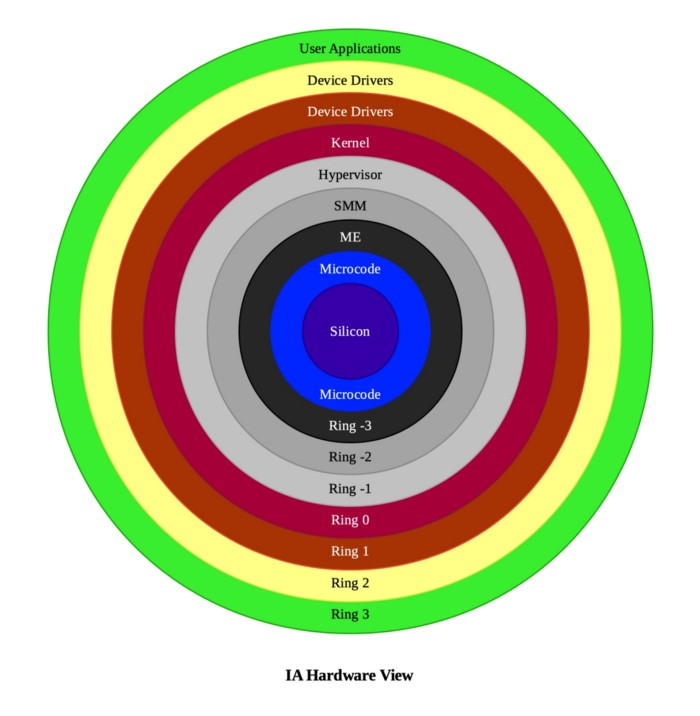
\includegraphics[width=.5\textwidth]{src/ring.jpeg}
    \caption{Intel Architecture Hardware View}
    \label{ring}
\end{figure}

Within the architecture of a computer system, a protection ring
\footnote{\url{https://www.eff.org/deeplinks/2017/05/intels-management-engine-security-hazard-and-users-need-way-disable-it}}
\footnote{\url{https://medium.com/swlh/negative-rings-in-intel-architecture-the-security-threats-youve-probably-never-heard-of-d725a4b6f831}}
, which is shown in figure \ref{ring}, is one of two or more
hierarchical levels or layers of privilege. Which was proposed by the Multics 
operating system \cite{6234805}.

Containers can theoretically have more secure ring protection in the
protection ring than in the host environment. Because the permitsions
of a container could have at most as many permissions as the host environment.
Therefore a container could break the protection ring, only if the host
machine could be cracked by those attacks which is applied in the container.

In other words, when a Container can break the protection ring, we permitted
too much capability to that container. Therefore, in our proposed method, the
system call limit during the container execution period is given at build time,
which can effectively defend against attacks such as breaking protection ring.

\subsection{Time Consuming}
\textcite{KOZHIRBAYEV2017175} showed that there is basically no
statistical difference between container and host environment.
This is completely in line with our perception of container, 
which is said that containers are isolated processes.

\subsection{Statistics}
According to our experiments, the integration tests and unit
tests were executed on IBM/FHIR server 4.9.0, and the system calls,
and system events we collected are shown in the figure \ref{hist}.

The figure \ref{hist} is the FHIR server's all system calls in
BoSC\cite{1495942} and the number of called times.
\begin{figure}
    \centering
    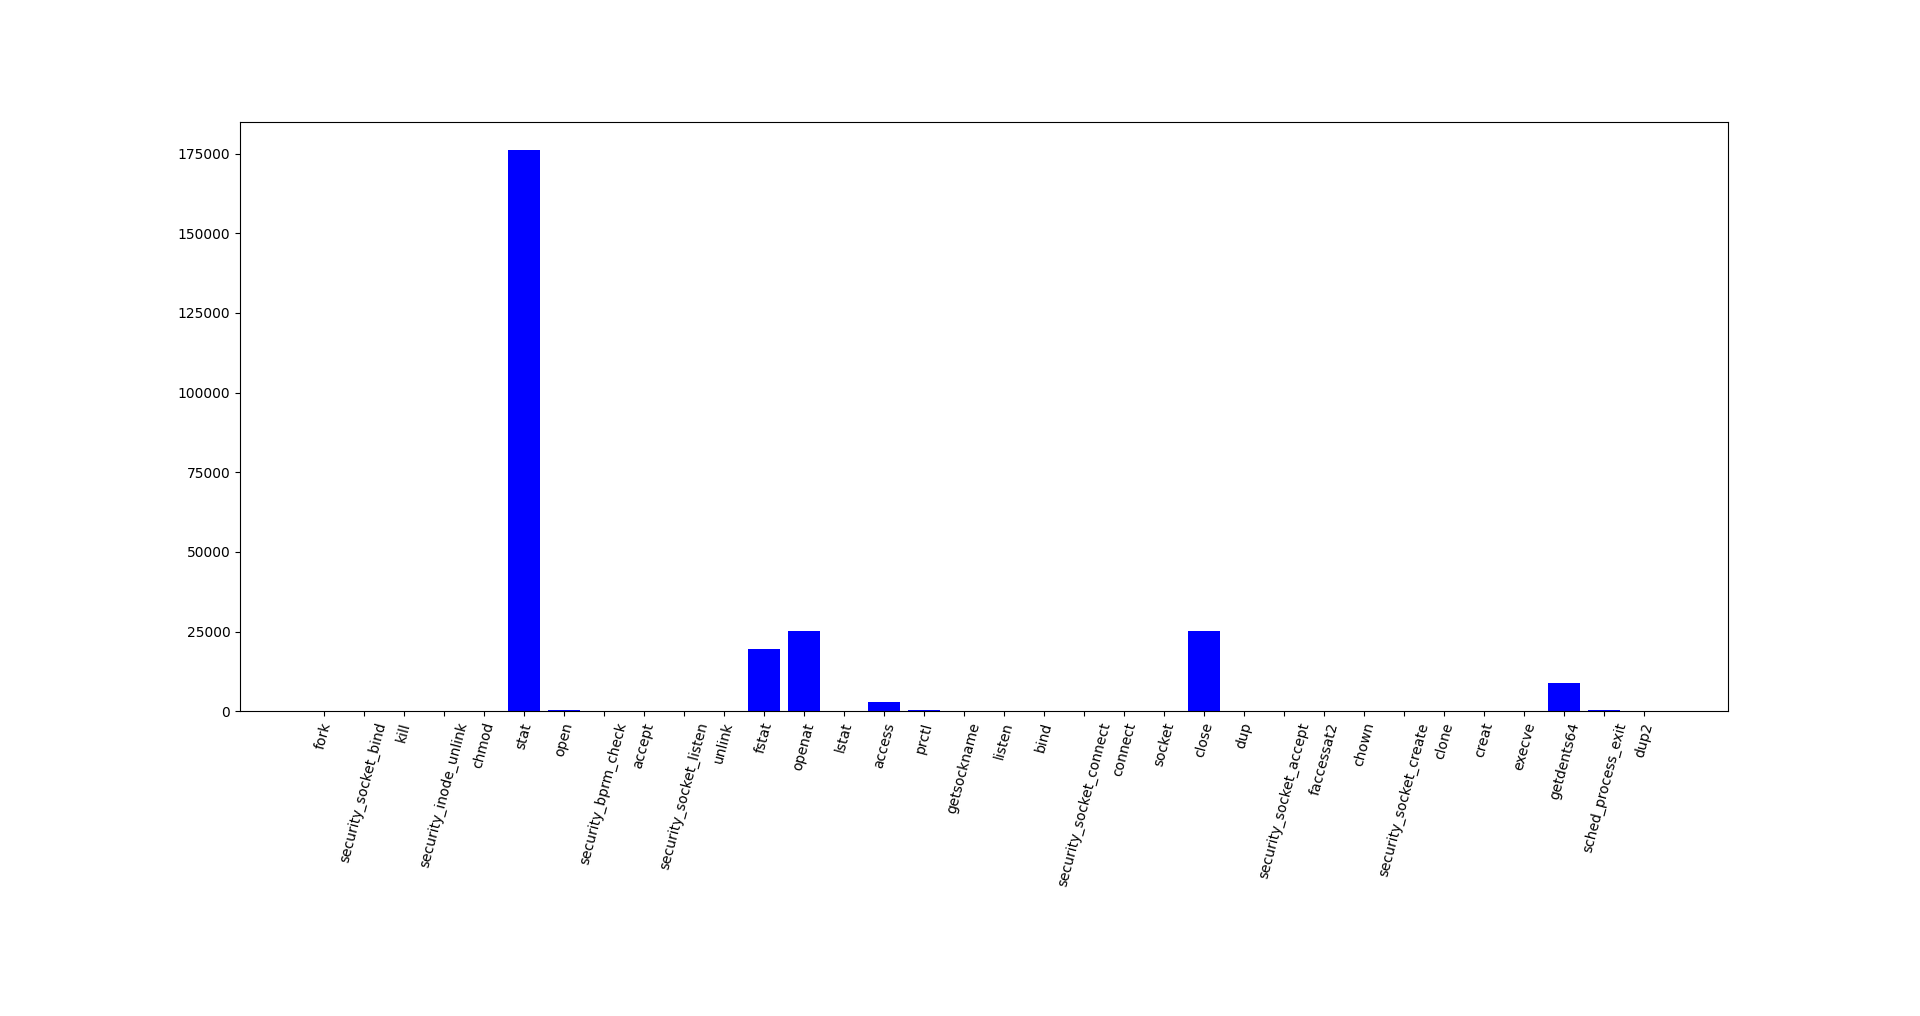
\includegraphics[width=\textwidth]{src/hist.png}
    \caption{All the system calls which the FHIR called times}
    \label{hist}
\end{figure}
Among them, we can find that the most used is the `stat' system call.


\section{Benchmark}
It is found that the discussion of container performance testing is less
focused on the requirement of parallel multiplexing
\cite{7371699,KOZHIRBAYEV2017175,7095802,234857}. And it is a more
important issue for the server's high multiplexing performance service client.

\subsection{Latency}
Figure \ref{conc} is the concurrent processes transporting time
difference in container and virtual machine.
\textcite{234857} showed that the latency of opening and closing files
are not significant difference between native and runc. But there was 12 times
faster than the gVisor with internal access. Although our IBM/FHIR server
cannot be executed in gVisor, it is the same in native and runc with no
significant difference.

\textcite{7095802} showd the relation between the throughput and the concurrency 
, both have transactions uppper bound cost in MySQL. The overhead of KVM is
much higher, above 40\% in all measured cases. We think there is a driver
buffering bottleneck in the hypervisior of KVM in ring 0.

So we compare the time lag between Ubuntu 20.04 in QEMU/KVM in Archlinux
and native Alpine container in Archlinux on concurrent requests. 
A phenomenon we found is that the latency curve of a virtual
machines seems to be different in complexity from that of a native container.

\begin{figure}
    \centering
    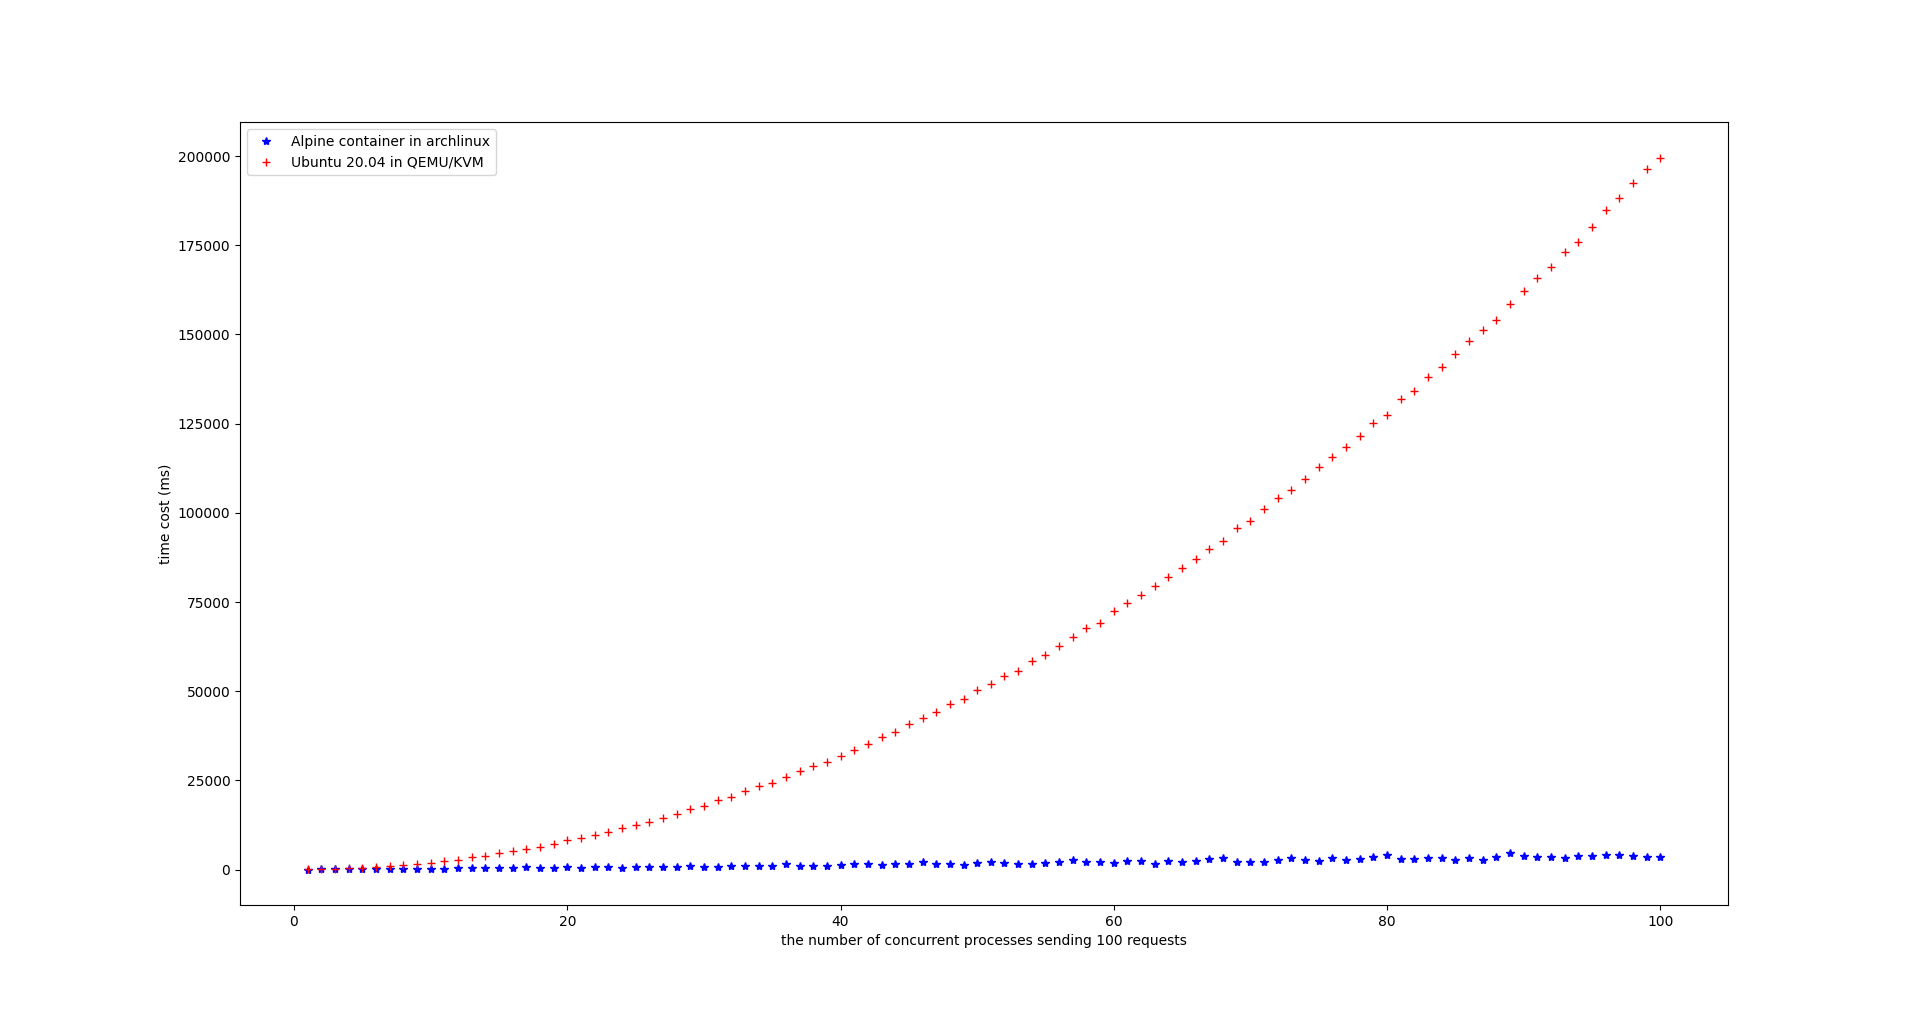
\includegraphics[width=\textwidth]{src/concurrent.png}
    \caption{Concurrent processes transporting time}
    \label{conc}
\end{figure}
